%% Robot PU 产品宣传册（中文版）— 2页，Letter纸，正反面打印
%% 编译方式：xelatex robotpu-brochure-cn.tex  （运行两次以更新交叉引用）
\documentclass[10pt]{article}

% ── 页面设置 ───────────────────────────────────────────────────────────────────
\usepackage[
  letterpaper,
  margin=0.45in,
  top=0.42in,
  bottom=0.42in
]{geometry}

% ── 中文支持（需要 XeLaTeX） ────────────────────────────────────────────────────
\usepackage{fontspec}
\usepackage{xeCJK}
\setCJKmainfont{Heiti SC}               % macOS 系统字体（黑体-简）
\setCJKsansfont{Heiti SC}
\setCJKmonofont{Heiti SC}
\setmainfont{Arial}                    % 西文字体
\setsansfont{Arial}

% ── 其他宏包 ───────────────────────────────────────────────────────────────────
\usepackage{xcolor}
\usepackage{graphicx}
\graphicspath{{./}{../}}
\usepackage{tikz}
\usepackage{multicol}
\usepackage{enumitem}
\usepackage{fontawesome5}
\usepackage{mdframed}
\usepackage{array}
\usepackage{tabularx}
\usepackage{booktabs}
\usepackage{parskip}
\usepackage{url}
\usepackage{tcolorbox}
\tcbuselibrary{skins,breakable}
\usepackage{wrapfig}
\usepackage{amssymb}
\usepackage{microtype}

% ── 颜色定义 ───────────────────────────────────────────────────────────────────
\definecolor{puBlue}{HTML}{1565C0}
\definecolor{puCyan}{HTML}{00B0FF}
\definecolor{puOrange}{HTML}{FF6D00}
\definecolor{puGray}{HTML}{455A64}
\definecolor{puLight}{HTML}{E3F2FD}
\definecolor{puDark}{HTML}{0D47A1}
\definecolor{puGreen}{HTML}{2E7D32}
\definecolor{puYellow}{HTML}{F9A825}
\definecolor{pageBg}{HTML}{F0F7FF}

% ── 不显示页码 ─────────────────────────────────────────────────────────────────
\pagestyle{empty}

% ── 自定义命令：彩色信息框 ──────────────────────────────────────────────────────
\newcommand{\featurebox}[3]{%
  \begin{tcolorbox}[
      colback=#1!8,
      colframe=#1,
      arc=3pt,
      boxrule=1pt,
      left=3pt, right=3pt, top=2pt, bottom=2pt,
      fonttitle=\bfseries\footnotesize\color{white},
      title={\textcolor{white}{#2}},
      coltitle=white,
      attach boxed title to top left={xshift=5pt,yshift=-2pt},
      boxed title style={colback=#1,arc=2pt}
    ]
    \footnotesize #3
  \end{tcolorbox}
}

% ── 文档开始 ───────────────────────────────────────────────────────────────────
\begin{document}

% ════════════════════════════════════════════════════════════════════════════════
%  第一页 — 产品概览
% ════════════════════════════════════════════════════════════════════════════════
\pagecolor{pageBg}

% ── 顶部标题栏 ─────────────────────────────────────────────────────────────────
\begin{tikzpicture}[remember picture, overlay]
  \fill[puDark] (current page.north west) rectangle
    ([yshift=-1.5cm]current page.north east);
  \node[anchor=west, xshift=0.55in, yshift=-0.75cm,
        text=white, font=\bfseries\Large] at (current page.north west)
    {Robot\,PU \quad\textcolor{puCyan}{|}\quad
     \textit{\normalsize 活泼可编程的 micro:bit 机器人}};
  \node[anchor=east, xshift=-0.55in, yshift=-0.75cm,
        text=white, font=\bfseries\small] at (current page.north east)
    {\textcolor{puYellow}{\faGlobe}\; robotgyms.com/pu};
\end{tikzpicture}

\vspace{1.4cm}

% ── 左图右文双栏布局 ──────────────────────────────────────────────────────────
\begin{minipage}[t]{0.48\linewidth}
  \vspace{0pt}
  \begin{center}
    \includegraphics[width=\linewidth,height=5.8cm,keepaspectratio]%
      {../product/robotpu.png}
  \end{center}
  \vspace{2pt}
  \begin{center}
    \includegraphics[width=0.55\linewidth,height=2.2cm,keepaspectratio]%
      {../product/robotpu_gamepad.png}\\[2pt]
    {\footnotesize\color{puGray} Robot PU 与手柄遥控器}
  \end{center}
\end{minipage}%
\hfill
\begin{minipage}[t]{0.49\linewidth}
  \vspace{0pt}

  % 标语
  {\large\bfseries\color{puDark}
   走路·跳舞·说话·导航·编程}

  \vspace{4pt}
  {\footnotesize\color{puGray}
  基于 \textbf{BBC micro:bit V2} 的完整课堂机器人套件。
  从小学课堂到大学机器人实验室，Robot PU 将抽象的 STEM 概念
  转化为生动有趣的实践项目。
  可选配 \textbf{ESP32-S3 智能帽}，解锁 AI 摄像头感知、
  足球对战与 SLAM 导航功能。}

  \vspace{5pt}

  % 套装内容
  \featurebox{puBlue}{\faBox\; 套装内容}{%
    \begin{itemize}[leftmargin=12pt, itemsep=0pt, topsep=0pt]
      \item Robot PU 机器人本体（预装可升级）
      \item 2 块 micro:bit 兼容主板
      \item 无线手柄遥控器
      \item 纸质说明书与快速入门指南
      \item 60+ 个在线教程、游戏与项目
    \end{itemize}
  }

  \vspace{4pt}

  % 编程路径
  \featurebox{puGreen}{\faCode\; 三种编程方式}{%
    \begin{tabularx}{\linewidth}{@{}lX@{}}
      \textbf{积木块} & MakeCode 图形化积木编程 \\
      \textbf{JS/TS}  & JavaScript / TypeScript 编程 \\
      \textbf{Python} & Python 扩展包（NovaSeq/RobotPu）\\
    \end{tabularx}
  }

  \vspace{4pt}

  % 可选配件
  \featurebox{puOrange}{\faMicrochip\; 可选升级：ESP32-S3 智能帽}{%
    新增 AI 摄像头、语音指令、SLAM 导航、人脸识别、
    目标追踪与足球自主对战功能。\textit{单独销售。}
  }
\end{minipage}

\vspace{5pt}
\noindent\textcolor{puCyan}{\rule{\linewidth}{1.5pt}}
\vspace{3pt}

% ── 四列功能展示 ───────────────────────────────────────────────────────────────
\begin{multicols}{4}

  % 第1列
  \begin{center}
    
\includegraphics[height=1.2cm,keepaspectratio]{../cartoons/pu_dance.png}
  \end{center}
  {\small\bfseries\color{puDark}行走与表达}\\
  {\footnotesize
    行走、转弯、横步、踢腿、跳跃、休息。
    随音乐节拍舞动。语音说话与唱歌，
    LED 眼睛显示情绪。}

  \columnbreak

  % 第2列
  \begin{center}
    
\includegraphics[height=1.2cm,keepaspectratio]{../cartoons/pu_walk.png}
  \end{center}
  {\small\bfseries\color{puDark}自动驾驶与导航}\\
  {\footnotesize
    超声波避障、迷宫求解、
    路径跟随、局部规划器、
    跟随领队、任务决策引擎。}

  \columnbreak

  % 第3列
  \begin{center}
    
\includegraphics[height=1.2cm,keepaspectratio]{../cartoons/pu_ideas.png}
  \end{center}
  {\small\bfseries\color{puDark}感知与控制}\\
  {\footnotesize
    超声波、IMU 姿态、
    罗盘航向、麦克风输入。
    信号滤波、航向融合、
    PID 平衡与舵机标定。}

  \columnbreak

  % 第4列
  \begin{center}
    
\includegraphics[height=1.2cm,keepaspectratio]{../cartoons/pu_star.png}
  \end{center}
  {\small\bfseries\color{puDark}多机器人与 AI}\\
  {\footnotesize
    无线手柄、点对点聊天、
    同步合唱、队形控制、
    任务分配、ROS 风格架构，
    AI 摄像头足球与 SLAM。}

\end{multicols}

\vspace{3pt}
\noindent\textcolor{puCyan}{\rule{\linewidth}{1pt}}
\vspace{2pt}

% ── 底部信息栏 ─────────────────────────────────────────────────────────────────
\begin{minipage}[c]{0.72\linewidth}
  \begin{tabular}{@{}ll@{}}
    \textcolor{puBlue}{\faShoppingCart} &
      \textbf{亚马逊购买：} \url{amazon.com/dp/B0DR8RGVXN} \\[3pt]
    \textcolor{puBlue}{\faGlobe} &
      \textbf{官方网站：} \url{robotgyms.com/pu} \\[3pt]
    \textcolor{puBlue}{\faYoutube} &
      \textbf{YouTube：} The Story of PU (\url{youtube.com/@TheStoryofPu-yw8tr}) \\[3pt]
    \textcolor{puBlue}{\faGithub} &
      \textbf{开源代码：} \url{github.com/robotgyms/pxt-robotpu} \\[3pt]
    \textcolor{puBlue}{\faMicrochip} &
      \textbf{MakeCode：} \url{makecode.microbit.org} — 添加扩展 \texttt{robotgyms/pxt-robotpu} \\
  \end{tabular}
\end{minipage}%
\hfill
\begin{minipage}[c]{0.25\linewidth}
  \begin{center}
    
\includegraphics[height=2.2cm,keepaspectratio]{../cartoons/pu_happy.png}\\
    {\footnotesize\color{puGray}\textit{来认识 PU！}}
  \end{center}
\end{minipage}

% ════════════════════════════════════════════════════════════════════════════════
%  第二页 — 教程内容
% ════════════════════════════════════════════════════════════════════════════════
\newpage
\pagecolor{pageBg}

% ── 顶部标题栏 ─────────────────────────────────────────────────────────────────
\begin{tikzpicture}[remember picture, overlay]
  \fill[puDark] (current page.north west) rectangle
    ([yshift=-1.5cm]current page.north east);
  \node[anchor=west, xshift=0.55in, yshift=-0.75cm,
        text=white, font=\bfseries\Large] at (current page.north west)
    {Robot\,PU \quad\textcolor{puCyan}{|}\quad
     \textit{\normalsize 60+ 个教程 — 从第一行代码到真实机器人}};
  \node[anchor=east, xshift=-0.55in, yshift=-0.75cm,
        text=white, font=\bfseries\small] at (current page.north east)
    {\textcolor{puYellow}{\faGlobe}\; robotgyms.com/pu};
\end{tikzpicture}

\vspace{1.4cm}

% ── 年龄段说明栏 ───────────────────────────────────────────────────────────────
\begin{tcolorbox}[
    colback=puDark,
    colframe=puDark,
    arc=6pt,
    left=8pt, right=8pt, top=5pt, bottom=5pt
  ]
  \centering
  \textcolor{white}{\bfseries\small
    {\color{puYellow}\faGraduationCap}\;
    8--10岁\,\textbf{入门} \quad
    \textcolor{puCyan}{$\bullet$} \quad
    11--13岁\,\textbf{进阶} \quad
    \textcolor{puCyan}{$\bullet$} \quad
    14--17岁\,\textbf{高级} \quad
    \textcolor{puCyan}{$\bullet$} \quad
    难度：
    {\color{puYellow}$\bigstar$} 入门\;
    {\color{puYellow}$\bigstar\bigstar$} 进阶\;
    {\color{puYellow}$\bigstar\bigstar\bigstar$} 高级}
\end{tcolorbox}

\vspace{4pt}

% ── 三栏教程列表 ───────────────────────────────────────────────────────────────
\begin{multicols}{3}

% ---- 第一栏 ------------------------------------------------------------------
\featurebox{puBlue}{\faRocket\; 环境搭建与基础}{%
  {\footnotesize
  \begin{tabular}{@{}p{0.06\linewidth}p{0.78\linewidth}@{}}
    {\color{puYellow}$\bigstar$}             & 项目骨架结构 \\
    {\color{puYellow}$\bigstar$}             & Hello World 演示程序 \\
    {\color{puYellow}$\bigstar\bigstar$}     & JavaScript / TypeScript 快速入门 \\
  \end{tabular}}
}

\vspace{3pt}

\featurebox{puBlue}{\faWrench\; 组装与标定}{%
  {\footnotesize
  \begin{tabular}{@{}p{0.06\linewidth}p{0.78\linewidth}@{}}
    {\color{puYellow}$\bigstar$} & 安装手臂 \\
    {\color{puYellow}$\bigstar$} & 舵机零点标定 \\
  \end{tabular}}
}

\vspace{3pt}

\featurebox{puBlue}{\faRunning\; 硬件与核心 API}{%
  {\footnotesize
  \begin{tabular}{@{}p{0.06\linewidth}p{0.78\linewidth}@{}}
    {\color{puYellow}$\bigstar$}             & PU 的运动原理 \\
    {\color{puYellow}$\bigstar$}             & 机器人动作指令 \\
    {\color{puYellow}$\bigstar\bigstar$}     & 机器人感知观测 \\
    {\color{puYellow}$\bigstar\bigstar$}     & 别撞墙（避障）\\
  \end{tabular}}
}

\vspace{3pt}

\featurebox{puGreen}{\faMusic\; 音乐、语音与表达}{%
  {\footnotesize
  \begin{tabular}{@{}p{0.06\linewidth}p{0.78\linewidth}@{}}
    {\color{puYellow}$\bigstar$}             & 音乐与节拍驱动行为 \\
    {\color{puYellow}$\bigstar$}             & 舞蹈编排 \\
    {\color{puYellow}$\bigstar\bigstar$}     & 音乐库工具 \\
    {\color{puYellow}$\bigstar\bigstar$}     & 情绪状态与表情 \\
    {\color{puYellow}$\bigstar\bigstar$}     & RoboVoice 旋律语音 \\
    {\color{puYellow}$\bigstar\bigstar$}     & 语音内容模板 \\
    {\color{puYellow}$\bigstar\bigstar$}     & 同步合唱 \\
  \end{tabular}}
}

\vspace{3pt}

\featurebox{puGreen}{\faGamepad\; 趣味项目}{%
  {\footnotesize
  \begin{tabular}{@{}p{0.06\linewidth}p{0.78\linewidth}@{}}
    {\color{puYellow}$\bigstar\bigstar$}         & 功夫动作序列 \\
    {\color{puYellow}$\bigstar\bigstar\bigstar$} & 学滑冰 \\
  \end{tabular}}
}

\columnbreak

% ---- 第二栏 ------------------------------------------------------------------
\featurebox{puOrange}{\faWifi\; 通信与控制}{%
  {\footnotesize
  \begin{tabular}{@{}p{0.06\linewidth}p{0.78\linewidth}@{}}
    {\color{puYellow}$\bigstar$}             & 遥控操作 \\
    {\color{puYellow}$\bigstar$}             & 手柄控制模式 \\
    {\color{puYellow}$\bigstar\bigstar$}     & 无线点对点聊天 \\
  \end{tabular}}
}

\vspace{3pt}

\featurebox{puOrange}{\faCodeBranch\; 程序结构}{%
  {\footnotesize
  \begin{tabular}{@{}p{0.06\linewidth}p{0.78\linewidth}@{}}
    {\color{puYellow}$\bigstar\bigstar$} & 事件循环 \\
    {\color{puYellow}$\bigstar\bigstar$} & 自定义事件与处理器 \\
    {\color{puYellow}$\bigstar\bigstar$} & 状态机 \\
    {\color{puYellow}$\bigstar\bigstar$} & 面向对象架构（OOP）\\
  \end{tabular}}
}

\vspace{3pt}

\featurebox{puOrange}{\faMap\; 导航、自主与建图}{%
  {\footnotesize
  \begin{tabular}{@{}p{0.06\linewidth}p{0.78\linewidth}@{}}
    {\color{puYellow}$\bigstar\bigstar$}         & 声呐操作 \\
    {\color{puYellow}$\bigstar\bigstar$}         & 迷宫求解 \\
    {\color{puYellow}$\bigstar\bigstar$}         & 自动驾驶导航 \\
    {\color{puYellow}$\bigstar\bigstar$}         & 二维建图概念 \\
    {\color{puYellow}$\bigstar\bigstar\bigstar$} & 潜水艇声呐项目 \\
    {\color{puYellow}$\bigstar\bigstar\bigstar$} & 跟随领队决策引擎 \\
    {\color{puYellow}$\bigstar\bigstar\bigstar$} & 占用格栅地图 \\
    {\color{puYellow}$\bigstar\bigstar\bigstar$} & 共享地图 \\
    {\color{puYellow}$\bigstar\bigstar\bigstar$} & 路径规划 \\
    {\color{puYellow}$\bigstar\bigstar\bigstar$} & 路径跟随 \\
    {\color{puYellow}$\bigstar\bigstar\bigstar$} & 局部规划器 \\
  \end{tabular}}
}

\vspace{3pt}

\begin{center}
  
\includegraphics[height=1.8cm,keepaspectratio]{../cartoons/pu_questions.png}
  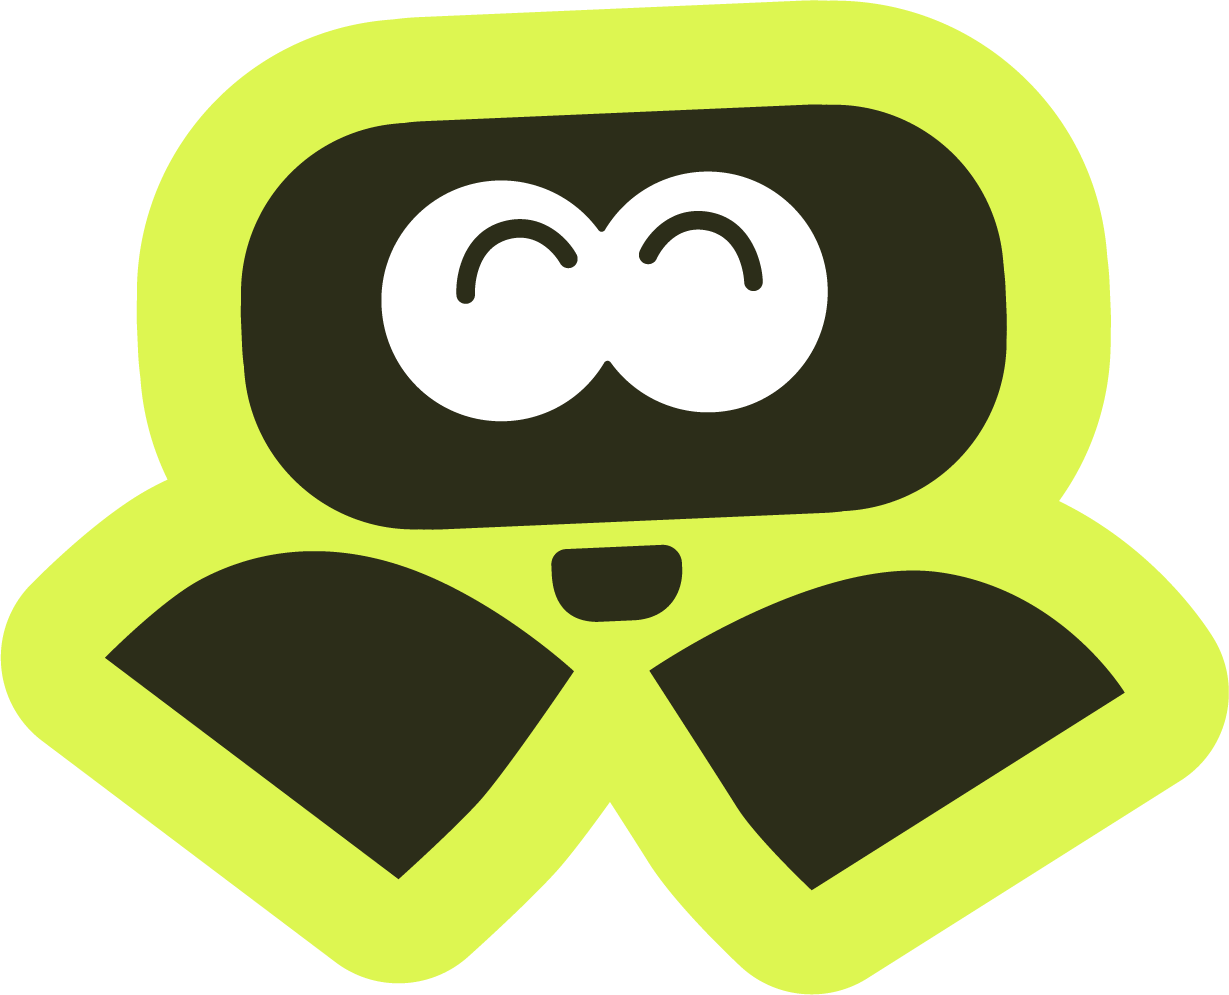
\includegraphics[height=1.8cm,keepaspectratio]{../cartoons/pu_jump.png}
\end{center}

\columnbreak

% ---- 第三栏 ------------------------------------------------------------------
\featurebox{puGray}{\faSitemap\; ROS 概念}{%
  {\footnotesize
  \begin{tabular}{@{}p{0.06\linewidth}p{0.78\linewidth}@{}}
    {\color{puYellow}$\bigstar\bigstar$}         & ROS 节点角色 \\
    {\color{puYellow}$\bigstar\bigstar$}         & micro:bit 上的 ROS 话题 \\
    {\color{puYellow}$\bigstar\bigstar$}         & /cmd\_vel 话题 \\
    {\color{puYellow}$\bigstar\bigstar$}         & /scan 话题 \\
    {\color{puYellow}$\bigstar\bigstar$}         & /diagnostics 话题 \\
    {\color{puYellow}$\bigstar\bigstar\bigstar$} & 遥测日志记录 \\
    {\color{puYellow}$\bigstar\bigstar\bigstar$} & 基站仪表盘 \\
    {\color{puYellow}$\bigstar\bigstar\bigstar$} & 安全守护 + 紧急停止 \\
    {\color{puYellow}$\bigstar\bigstar\bigstar$} & 故障恢复行为 \\
    {\color{puYellow}$\bigstar\bigstar\bigstar$} & 行为树 \\
    {\color{puYellow}$\bigstar\bigstar\bigstar$} & 任务配方 \\
    {\color{puYellow}$\bigstar\bigstar\bigstar$} & 任务分配 \\
    {\color{puYellow}$\bigstar\bigstar\bigstar$} & 队形控制 \\
  \end{tabular}}
}

\vspace{3pt}

\featurebox{puGray}{\faCalculator\; 控制理论与数学}{%
  {\footnotesize
  \begin{tabular}{@{}p{0.06\linewidth}p{0.78\linewidth}@{}}
    {\color{puYellow}$\bigstar\bigstar\bigstar$} & 变换矩阵 \\
    {\color{puYellow}$\bigstar\bigstar\bigstar$} & 反馈控制回路 \\
    {\color{puYellow}$\bigstar\bigstar\bigstar$} & 信号滤波器 \\
    {\color{puYellow}$\bigstar\bigstar\bigstar$} & 航向融合 \\
    {\color{puYellow}$\bigstar\bigstar\bigstar$} & PID 平衡控制 \\
    {\color{puYellow}$\bigstar\bigstar\bigstar$} & 高级平衡控制 \\
  \end{tabular}}
}

\vspace{3pt}

\featurebox{puOrange}{\faCamera\; 视觉、AI 与足球 SLAM}{%
  {\footnotesize
  \begin{tabular}{@{}p{0.06\linewidth}p{0.78\linewidth}@{}}
    {\color{puYellow}$\bigstar\bigstar\bigstar$} & K230 AI 摄像头 \\
    {\color{puYellow}$\bigstar\bigstar\bigstar$} & 人脸搜索与追踪 \\
    {\color{puYellow}$\bigstar\bigstar\bigstar$} & SLAM I2C 摄像头消息 \\
    {\color{puYellow}$\bigstar\bigstar\bigstar$} & SLAM 里程计 \\
    {\color{puYellow}$\bigstar\bigstar\bigstar$} & SLAM 足球追踪 \\
    {\color{puYellow}$\bigstar\bigstar\bigstar$} & SLAM 足球局部地图 \\
  \end{tabular}}
}

\end{multicols}

\vspace{2pt}
\noindent\textcolor{puCyan}{\rule{\linewidth}{1pt}}
\vspace{2pt}

% ── 底部信息栏 ─────────────────────────────────────────────────────────────────
\begin{minipage}[c]{0.32\linewidth}
  \begin{center}
    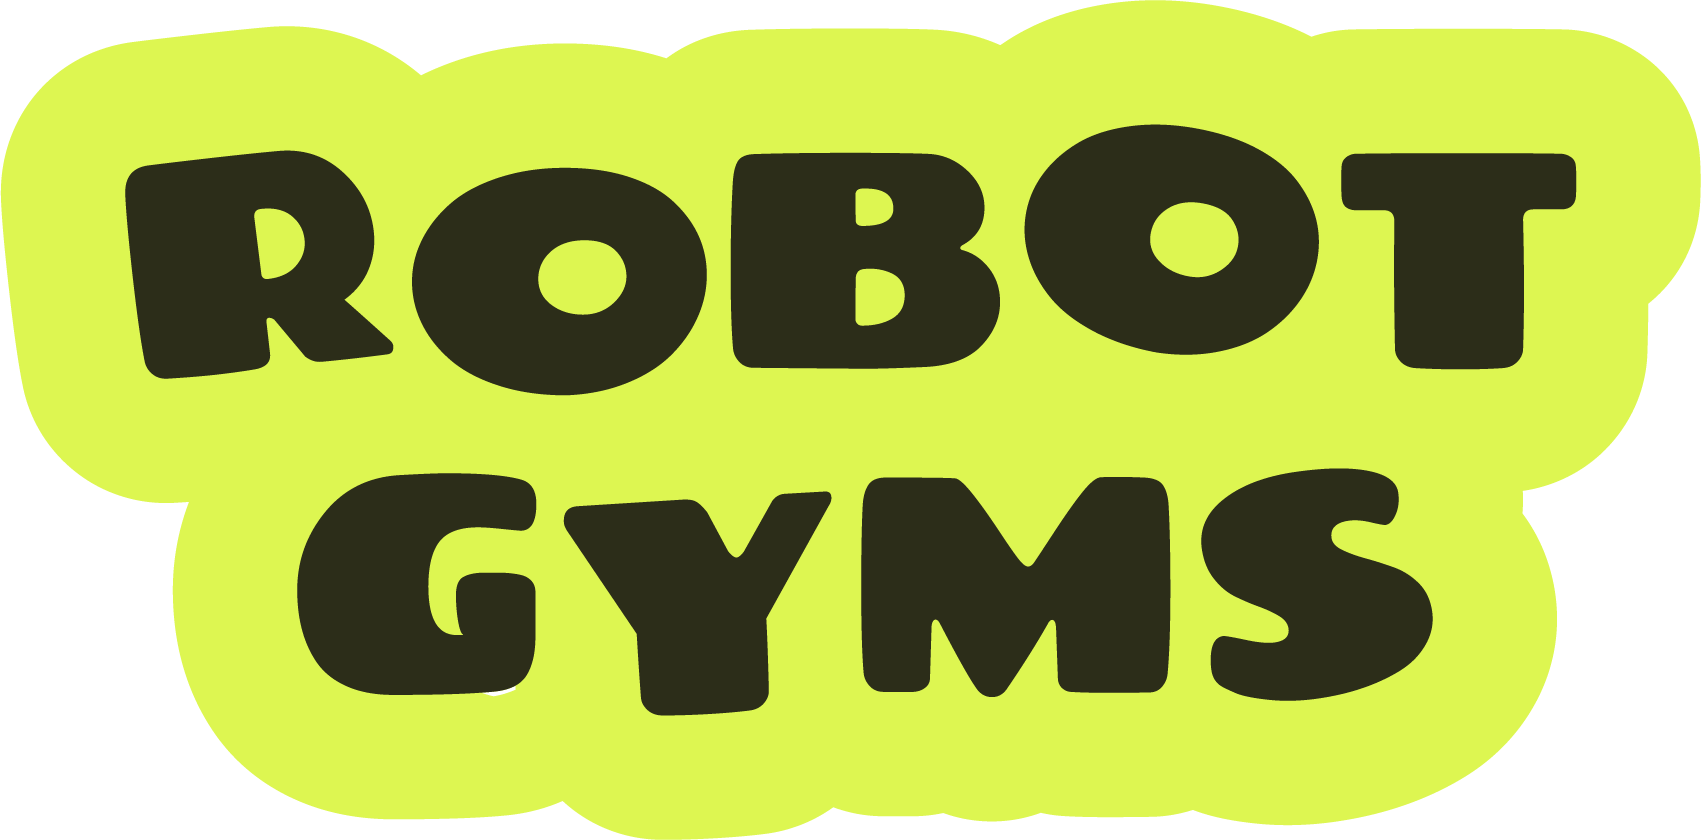
\includegraphics[height=1.6cm,keepaspectratio]{../brand/robotgyms_logo.png}
  \end{center}
\end{minipage}%
\hfill
\begin{minipage}[c]{0.35\linewidth}
  \centering
  {\small\bfseries\color{puDark}PU 的故事 — 系列学习书籍}\\[3pt]
  {\footnotesize
  \textcolor{puBlue}{第一册} 配对启航 \;|\;
  \textcolor{puBlue}{第二册} 游戏 \;|\;
  \textcolor{puBlue}{第三册} 成长\\
  \textcolor{puBlue}{第四册} 旅程 \;|\;
  \textcolor{puBlue}{第五册} AI 摄像头\\[3pt]
  \url{robotgyms.com/pu}}
\end{minipage}%
\hfill
\begin{minipage}[c]{0.28\linewidth}
  \begin{center}
    
\includegraphics[height=1.6cm,keepaspectratio]{../cartoons/pu_sing.png}
    
\includegraphics[height=1.6cm,keepaspectratio]{../cartoons/pu_supprise.png}
  \end{center}
\end{minipage}

\end{document}
